\documentclass[10pt]{beamer}

\useoutertheme[footline=authortitle]{miniframes}

\usepackage[utf8]{inputenc}
\usepackage{amsmath}
\usepackage{amsfonts}
\usepackage{amssymb}
\usepackage{gensymb}
\usepackage{graphicx}
\usepackage{svg}
\author{Thomas Parry}
\title{Amateur Radio Satellite Transceiver (SKY130)}

\setbeamertemplate{items}[square]
\setbeamertemplate{itemize/enumerate body begin}{\footnotesize}


\setbeamertemplate{section page}
{
  \begingroup
    \centering
%    {\usebeamerfont{section name}\usebeamercolor[fg]{section name}\sectionname~\insertsectionnumber}
    \vskip1em\par
    \begin{beamercolorbox}[sep=12pt,center,colsep=-4bp,rounded=true,shadow=\beamer@themerounded@shadow]{section title}
      \usebeamerfont{section title}\insertsection\par
    \end{beamercolorbox}
  \endgroup
}

\setbeamertemplate{subsection page}
{
  \begingroup
    \centering
%    {\usebeamerfont{section name}\usebeamercolor[fg]{section name}\sectionname~\insertsectionnumber}
    \vskip1em\par
    \begin{beamercolorbox}[sep=12pt,center,colsep=-4bp,rounded=true,shadow=\beamer@themerounded@shadow]{subsection title}
      \usebeamerfont{subsection title}\insertsubsection\par
    \end{beamercolorbox}
  \endgroup
}






\begin{document}


%%%%%%%%%%%%%%%%%%%%%%%%%%%%%%%%%%%%%%%%%%%%%%%%%%%%%%%%%%%%%%%%%%%%%%%%%%%%%%%%%%%%%%%%%%%%%%%%%%%%%%%%%%%%%%
\begin{frame}
\titlepage
\end{frame}

%%%%%%%%%%%%%%%%%%%%%%%%%%%%%%%%%%%%%%%%%%%%%%%%%%%%%%%%%%%%%%%%%%%%%%%%%%%%%%%%%%%%%%%%%%%%%%%%%%%%%%%%%%%%%%
%%%%%%%%%%%%%%%%%%%%%%%%%%%%%%%%%%%%%%%%%%%%%%%%%%%%%%%%%%%%%%%%%%%%%%%%%%%%%%%%%%%%%%%%%%%%%%%%%%%%%%%%%%%%%%
\section{Objectives}

%%%%%%%%%%%%%%%%%%%%%%%%%%%%%%%%%%%%%%%%%%%%%%%%%%%%%%%%%%%%%%%%%%%%%%%%%%%%%%%%%%%%%%%%%%%%%%%%%%%%%%%%%%%%%%
\begin{frame}{System Goal}

\begin{figure}[h]
\centering{
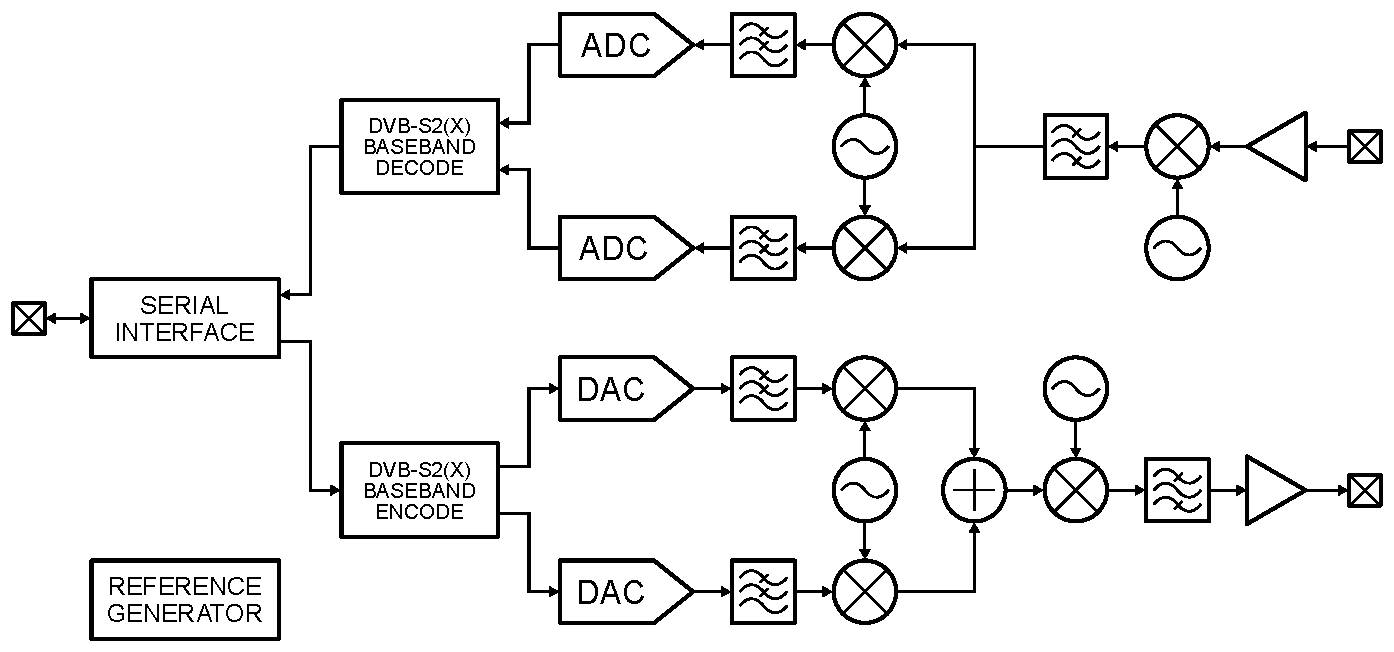
\includegraphics[scale=0.4]{system}
}
\end{figure}

\begin{itemize}
 \item Amateur radio satellite transceiver
 \item Microwave bands - 2.4 GHz, 5.8 GHz and 10.2 GHz
 \item Payload data to antenna and back
\end{itemize}

\end{frame}


%%%%%%%%%%%%%%%%%%%%%%%%%%%%%%%%%%%%%%%%%%%%%%%%%%%%%%%%%%%%%%%%%%%%%%%%%%%%%%%%%%%%%%%%%%%%%%%%%%%%%%%%%%%%%%
%%%%%%%%%%%%%%%%%%%%%%%%%%%%%%%%%%%%%%%%%%%%%%%%%%%%%%%%%%%%%%%%%%%%%%%%%%%%%%%%%%%%%%%%%%%%%%%%%%%%%%%%%%%%%%
\section*{MPW-A}
\frame{\sectionpage}

%%%%%%%%%%%%%%%%%%%%%%%%%%%%%%%%%%%%%%%%%%%%%%%%%%%%%%%%%%%%%%%%%%%%%%%%%%%%%%%%%%%%%%%%%%%%%%%%%%%%%%%%%%%%%%
\begin{frame}{System View}

\begin{figure}[h]
\centering{
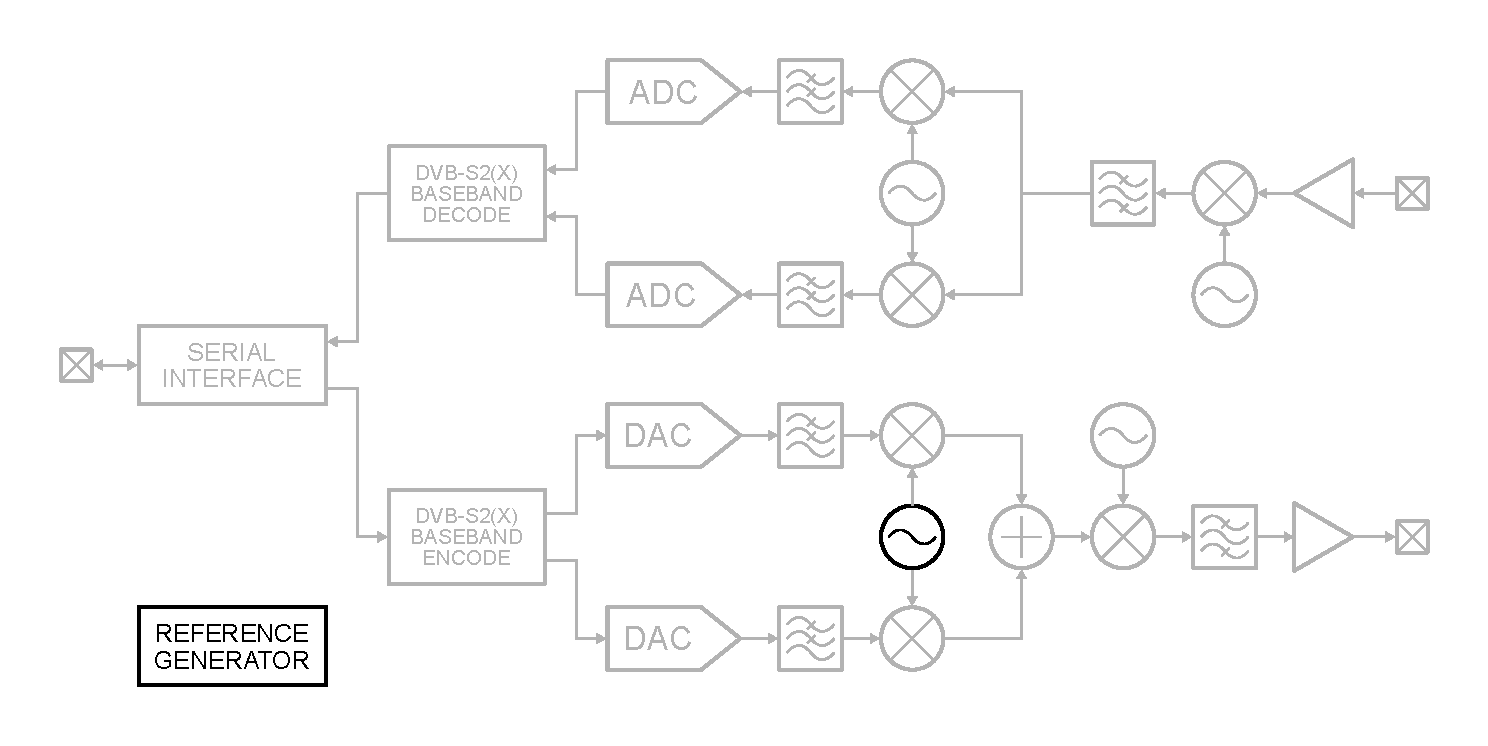
\includegraphics[scale=0.4]{system_mpw-a}
}
\end{figure}

\end{frame}


\subsection{Bandgap Reference}

%%%%%%%%%%%%%%%%%%%%%%%%%%%%%%%%%%%%%%%%%%%%%%%%%%%%%%%%%%%%%%%%%%%%%%%%%%%%%%%%%%%%%%%%%%%%%%%%%%%%%%%%%%%%%%
\begin{frame}{Bandgap Topology}

\begin{figure}[h]
\centering{
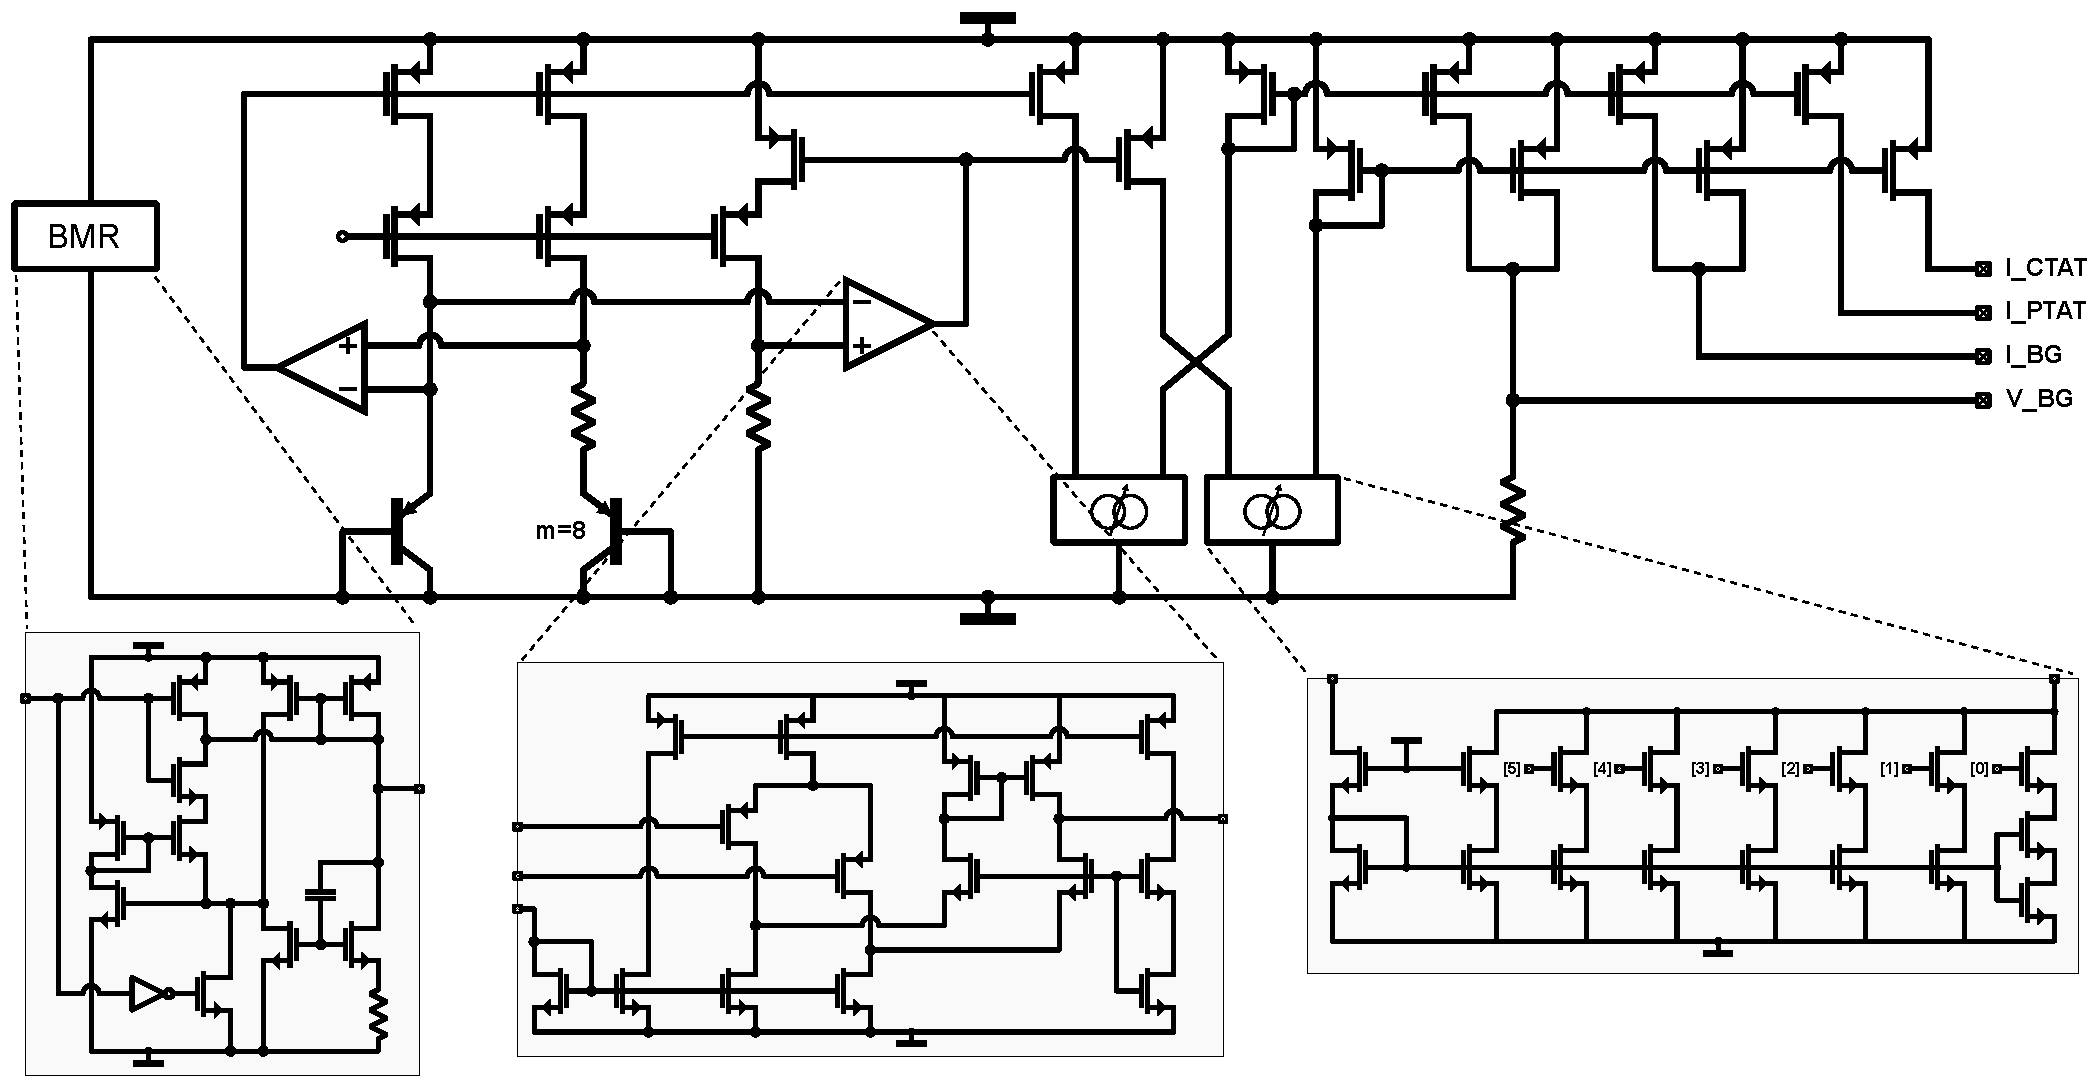
\includegraphics[scale=0.25]{bandgap_topology_full}
}
\end{figure}

\begin{itemize}
 \item Separate PTAT and CTAT with 6-bits trimming
 \item Less than $\pm 0.2 \% $ variation from $-40 ^{\circ}$ to $125 ^{\circ}$
\end{itemize}

\end{frame}


%%%%%%%%%%%%%%%%%%%%%%%%%%%%%%%%%%%%%%%%%%%%%%%%%%%%%%%%%%%%%%%%%%%%%%%%%%%%%%%%%%%%%%%%%%%%%%%%%%%%%%%%%%%%%%
\begin{frame}{Bandgap Layout}
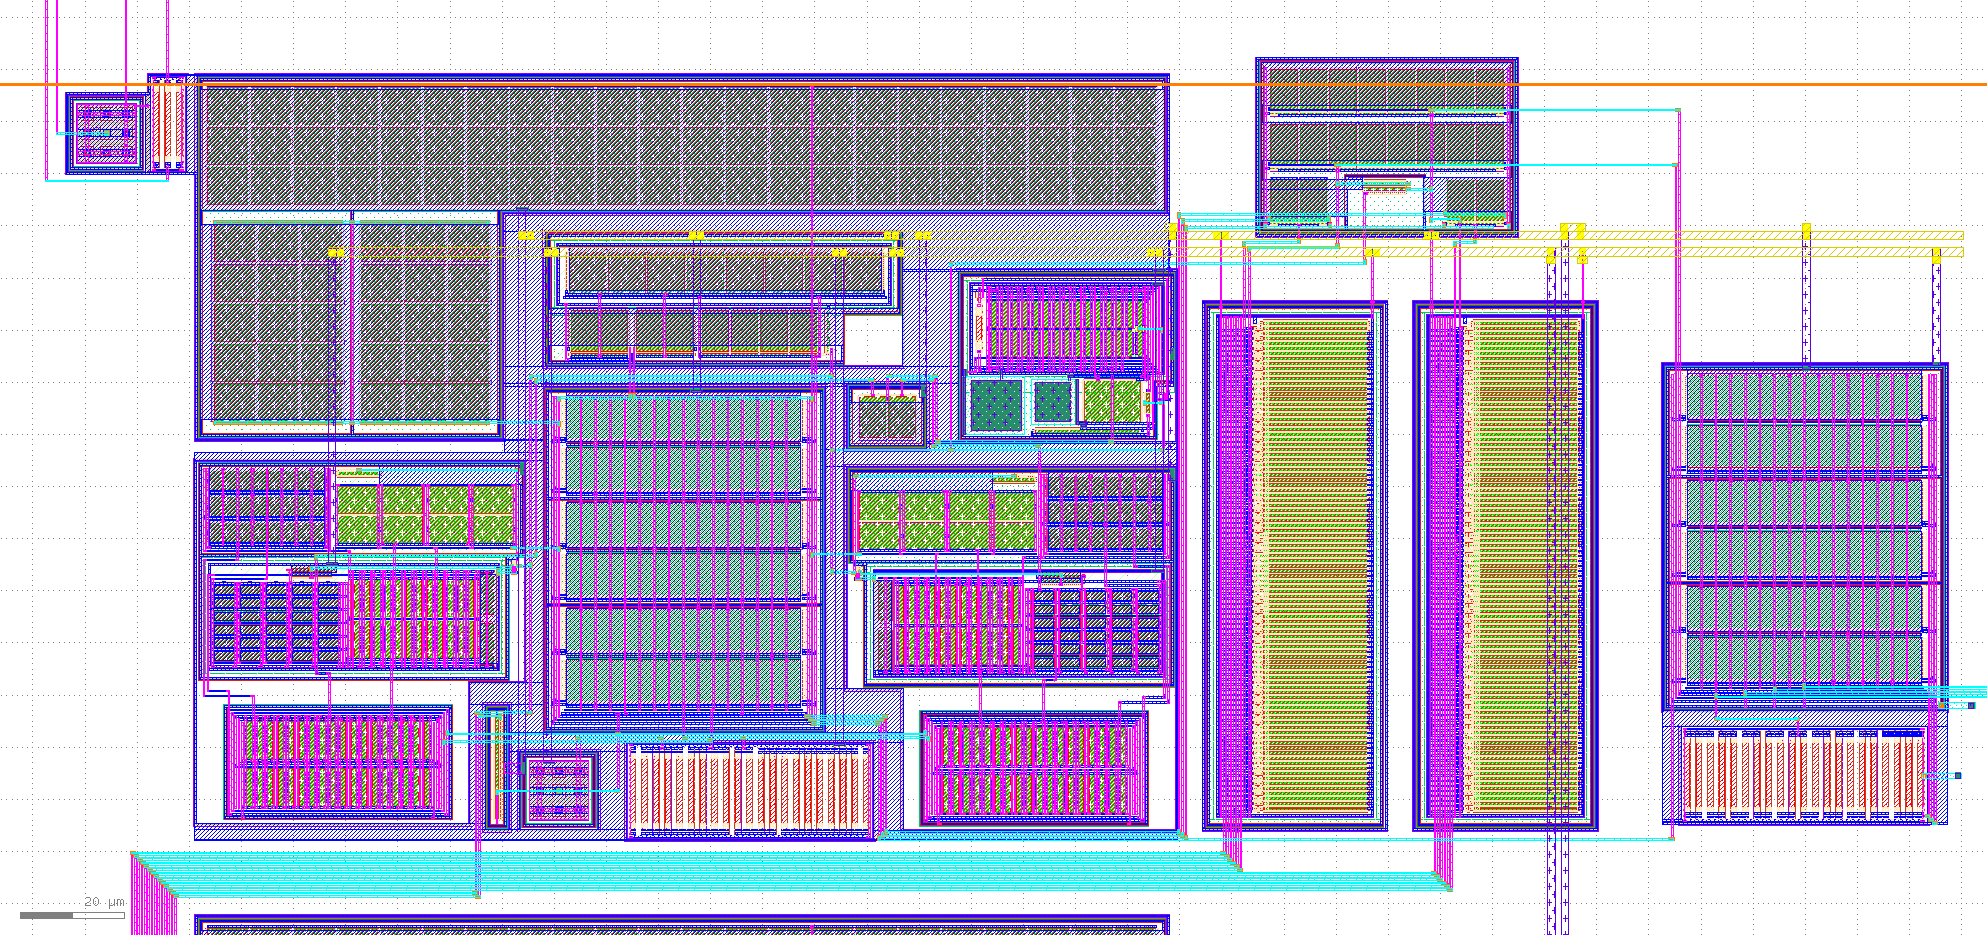
\includegraphics[scale=0.18]{bandgap_layout}
\end{frame}


%%%%%%%%%%%%%%%%%%%%%%%%%%%%%%%%%%%%%%%%%%%%%%%%%%%%%%%%%%%%%%%%%%%%%%%%%%%%%%%%%%%%%%%%%%%%%%%%%%%%%%%%%%%%%%
%%%%%%%%%%%%%%%%%%%%%%%%%%%%%%%%%%%%%%%%%%%%%%%%%%%%%%%%%%%%%%%%%%%%%%%%%%%%%%%%%%%%%%%%%%%%%%%%%%%%%%%%%%%%%%
\subsection{Phase Locked Loop}

%%%%%%%%%%%%%%%%%%%%%%%%%%%%%%%%%%%%%%%%%%%%%%%%%%%%%%%%%%%%%%%%%%%%%%%%%%%%%%%%%%%%%%%%%%%%%%%%%%%%%%%%%%%%%%
\begin{frame}{PLL Topology}

\begin{figure}[h]
\centering{
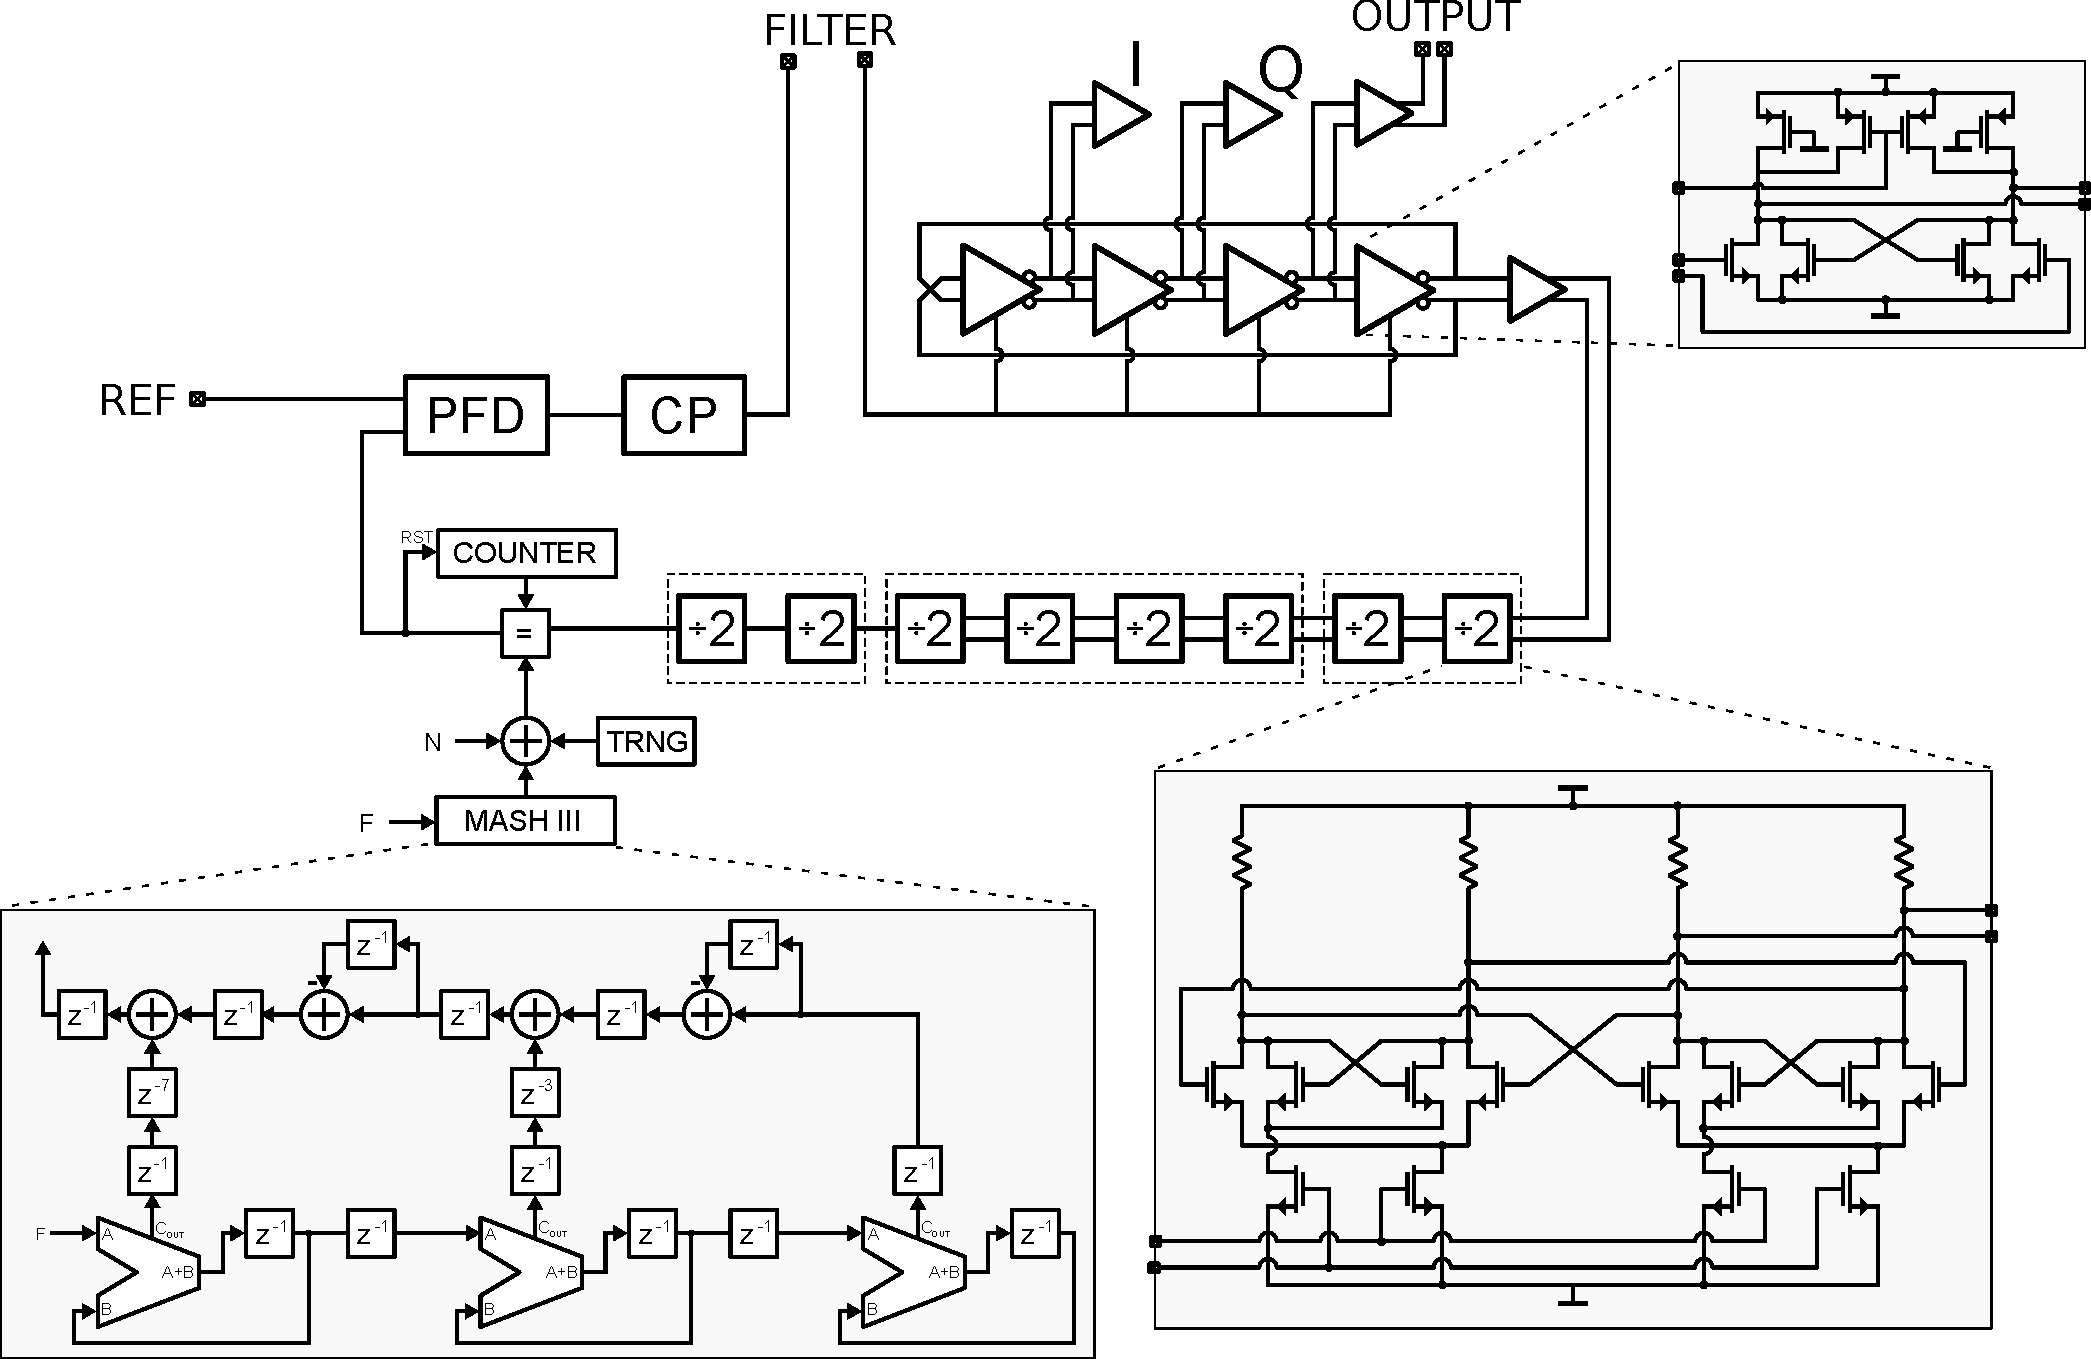
\includegraphics[scale=0.24]{pll_topology.pdf}
}
\end{figure}

\begin{itemize}
 \item 1.3 - 3.6 GHz differential quadrature output range
 \item CML and FF pre-scalars, third-order MASH modulator with TRNG dither
 \item Off chip compensation filter
\end{itemize}

\end{frame}


%%%%%%%%%%%%%%%%%%%%%%%%%%%%%%%%%%%%%%%%%%%%%%%%%%%%%%%%%%%%%%%%%%%%%%%%%%%%%%%%%%%%%%%%%%%%%%%%%%%%%%%%%%%%%%
\begin{frame}{PLL Layout}
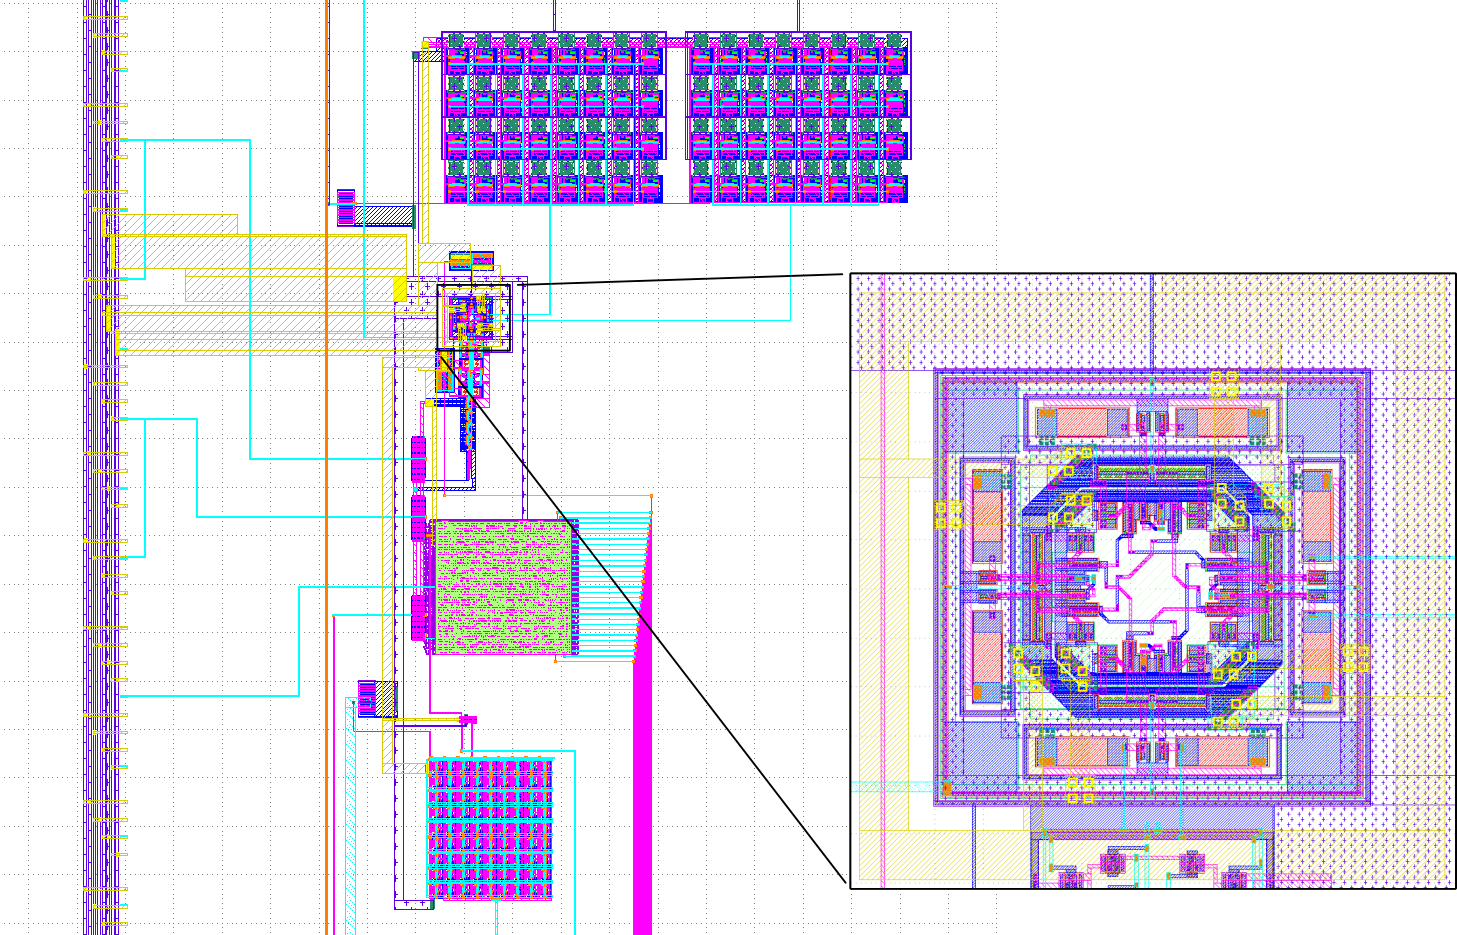
\includegraphics[scale=0.25]{pll_vco_layout}
\end{frame}



%%%%%%%%%%%%%%%%%%%%%%%%%%%%%%%%%%%%%%%%%%%%%%%%%%%%%%%%%%%%%%%%%%%%%%%%%%%%%%%%%%%%%%%%%%%%%%%%%%%%%%%%%%%%%%
%%%%%%%%%%%%%%%%%%%%%%%%%%%%%%%%%%%%%%%%%%%%%%%%%%%%%%%%%%%%%%%%%%%%%%%%%%%%%%%%%%%%%%%%%%%%%%%%%%%%%%%%%%%%%%
\subsection*{Tools}

\frame{\subsectionpage}

%%%%%%%%%%%%%%%%%%%%%%%%%%%%%%%%%%%%%%%%%%%%%%%%%%%%%%%%%%%%%%%%%%%%%%%%%%%%%%%%%%%%%%%%%%%%%%%%%%%%%%%%%%%%%%
\begin{frame}{Schematic Capture}

\begin{figure}[h]
\centering{
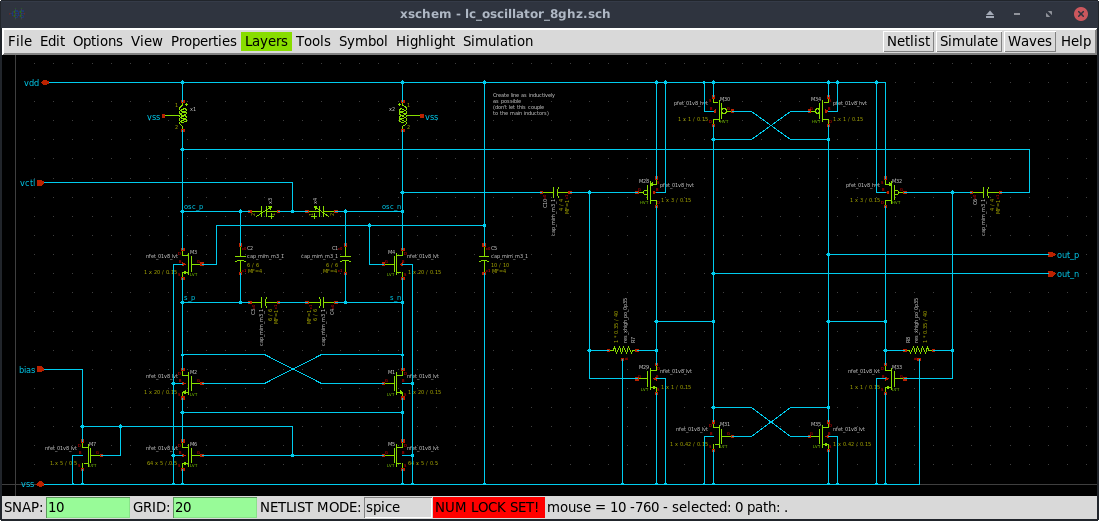
\includegraphics[scale=0.25]{xschem.png}
}
\end{figure}

\centering{
\tiny xschem - github.com/StefanSchippers/xschem
}

\end{frame}

%%%%%%%%%%%%%%%%%%%%%%%%%%%%%%%%%%%%%%%%%%%%%%%%%%%%%%%%%%%%%%%%%%%%%%%%%%%%%%%%%%%%%%%%%%%%%%%%%%%%%%%%%%%%%%
\begin{frame}{Layout}

\begin{figure}[h]
\centering{
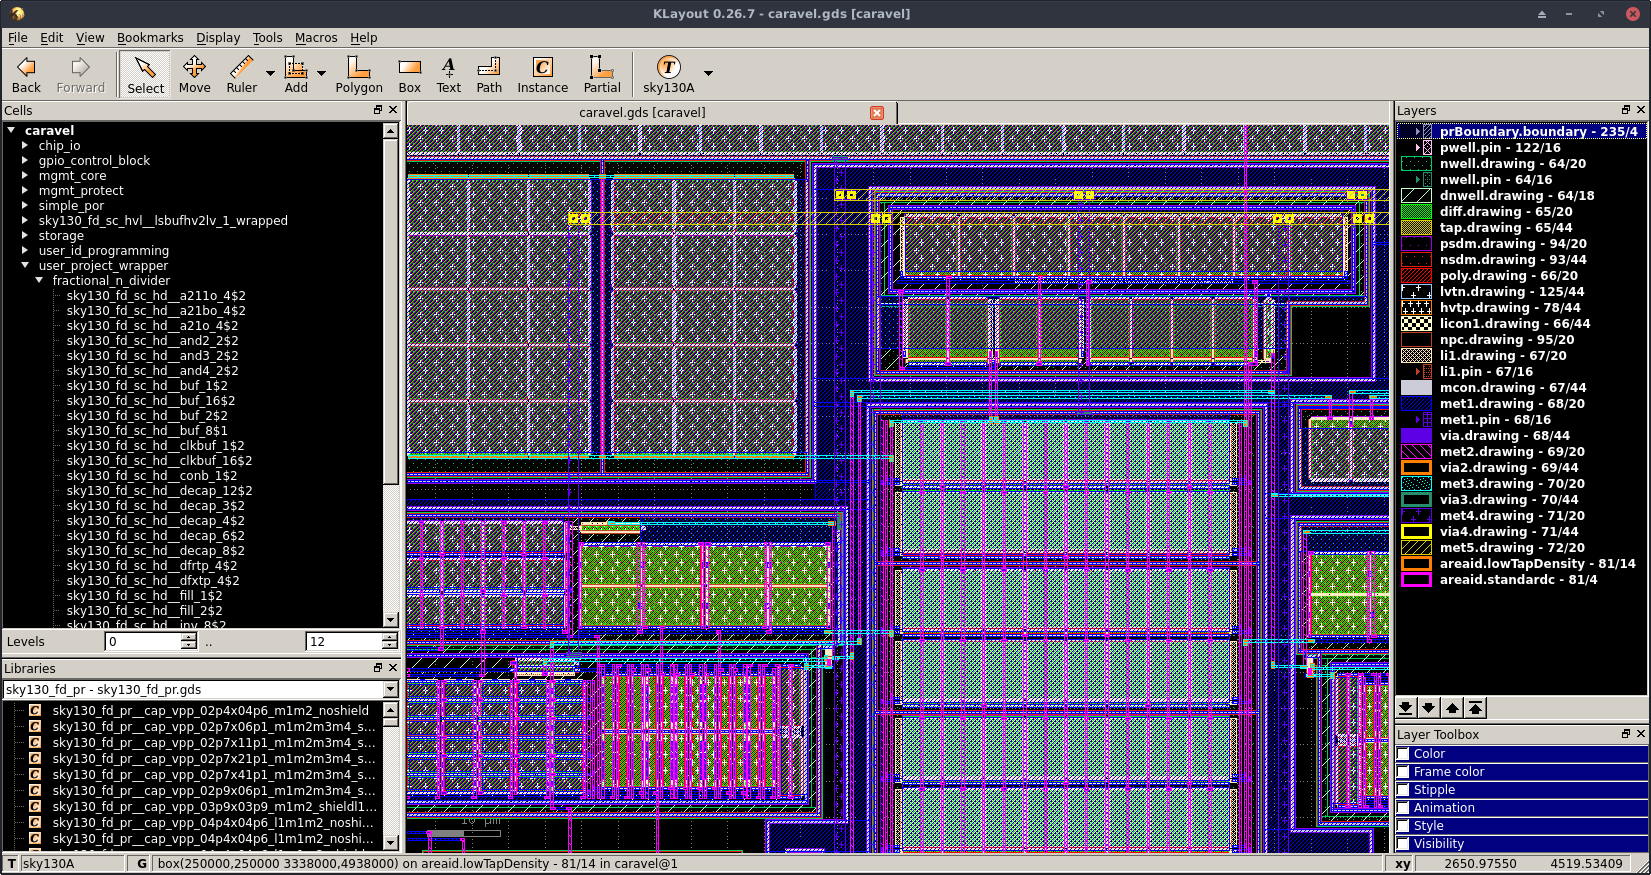
\includegraphics[scale=0.16]{klayout.png}
}
\end{figure}

\centering{
\tiny KLayout - klayout.de \\
\tiny Magic - opencircuitdesign.com/magic
}

\end{frame}


%%%%%%%%%%%%%%%%%%%%%%%%%%%%%%%%%%%%%%%%%%%%%%%%%%%%%%%%%%%%%%%%%%%%%%%%%%%%%%%%%%%%%%%%%%%%%%%%%%%%%%%%%%%%%%
\begin{frame}{Simulation}

\begin{columns}

\column{0.7\textwidth}
Open source Spice simulators:
\begin{itemize}
\item NGSpice
\item Xyce
\end{itemize}

Command line interface only

\column{0.3\textwidth}

\begin{figure}[h]
\centering{

\includegraphics[scale=0.25]{nglogo.jpg}

\includegraphics[scale=0.25]{xyce.png}
}
\end{figure}

\end{columns}
\end{frame}

%%%%%%%%%%%%%%%%%%%%%%%%%%%%%%%%%%%%%%%%%%%%%%%%%%%%%%%%%%%%%%%%%%%%%%%%%%%%%%%%%%%%%%%%%%%%%%%%%%%%%%%%%%%%%%
\begin{frame}{Python}

\begin{columns}

\column{0.7\textwidth}

Components plugged together using Python.

\begin{itemize}
\item Device characterisation and querying
\item Automated simulation
\item Post-processing measurement
\item Unit tests (OpenHTF / pytest)
\end{itemize}

\column{0.3\textwidth}
\begin{figure}[h]
\centering{

\includegraphics[scale=0.05]{python.png}
}
\end{figure}

\end{columns}

\end{frame}


%%%%%%%%%%%%%%%%%%%%%%%%%%%%%%%%%%%%%%%%%%%%%%%%%%%%%%%%%%%%%%%%%%%%%%%%%%%%%%%%%%%%%%%%%%%%%%%%%%%%%%%%%%%%%%
%%%%%%%%%%%%%%%%%%%%%%%%%%%%%%%%%%%%%%%%%%%%%%%%%%%%%%%%%%%%%%%%%%%%%%%%%%%%%%%%%%%%%%%%%%%%%%%%%%%%%%%%%%%%%%
\section*{MPW-B}
\frame{\sectionpage}

%%%%%%%%%%%%%%%%%%%%%%%%%%%%%%%%%%%%%%%%%%%%%%%%%%%%%%%%%%%%%%%%%%%%%%%%%%%%%%%%%%%%%%%%%%%%%%%%%%%%%%%%%%%%%%
\begin{frame}{Aim}

\begin{figure}[h]
\centering{
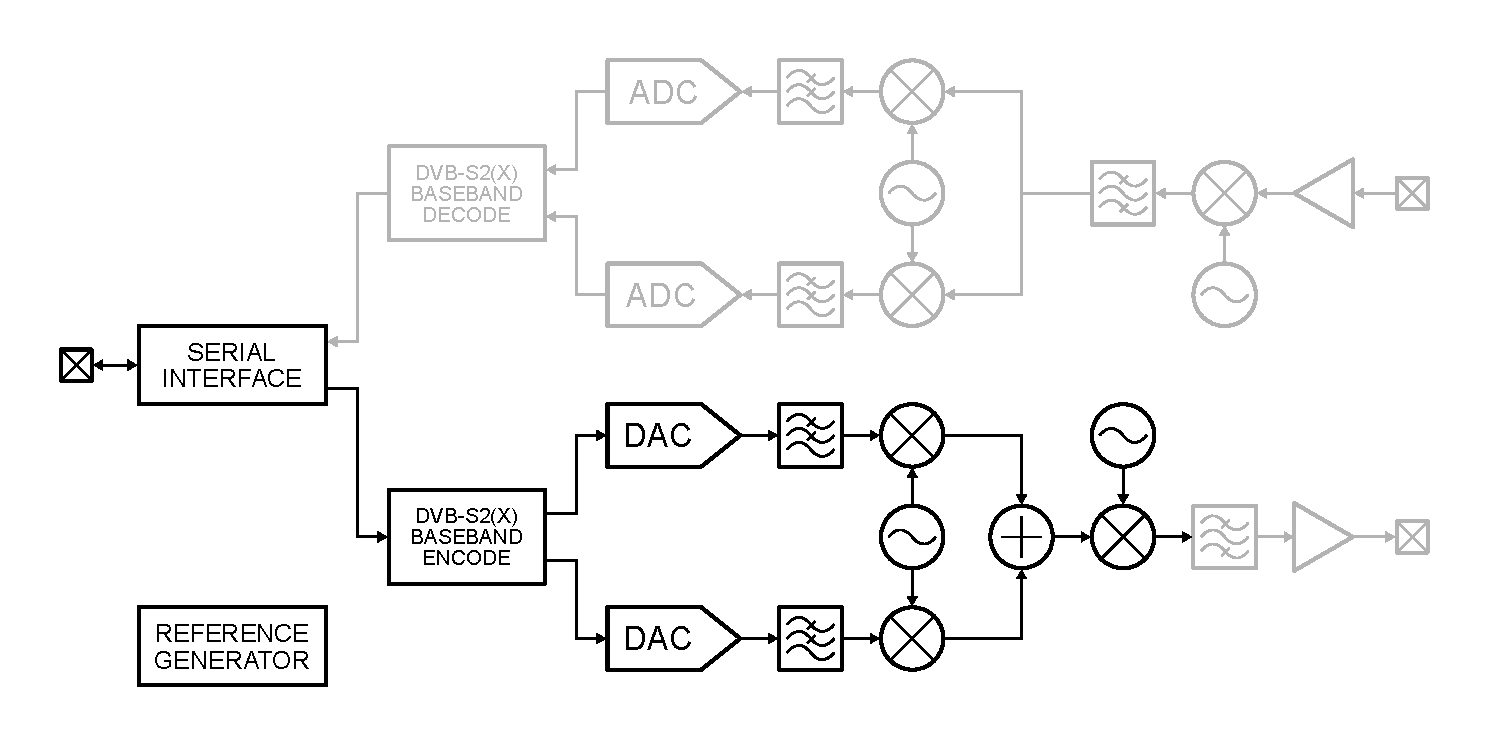
\includegraphics[scale=0.4]{system_mpw-b}
}
\end{figure}

\end{frame}


%%%%%%%%%%%%%%%%%%%%%%%%%%%%%%%%%%%%%%%%%%%%%%%%%%%%%%%%%%%%%%%%%%%%%%%%%%%%%%%%%%%%%%%%%%%%%%%%%%%%%%%%%%%%%%
\begin{frame}{DAC Topology}

\begin{figure}[h]
\centering{
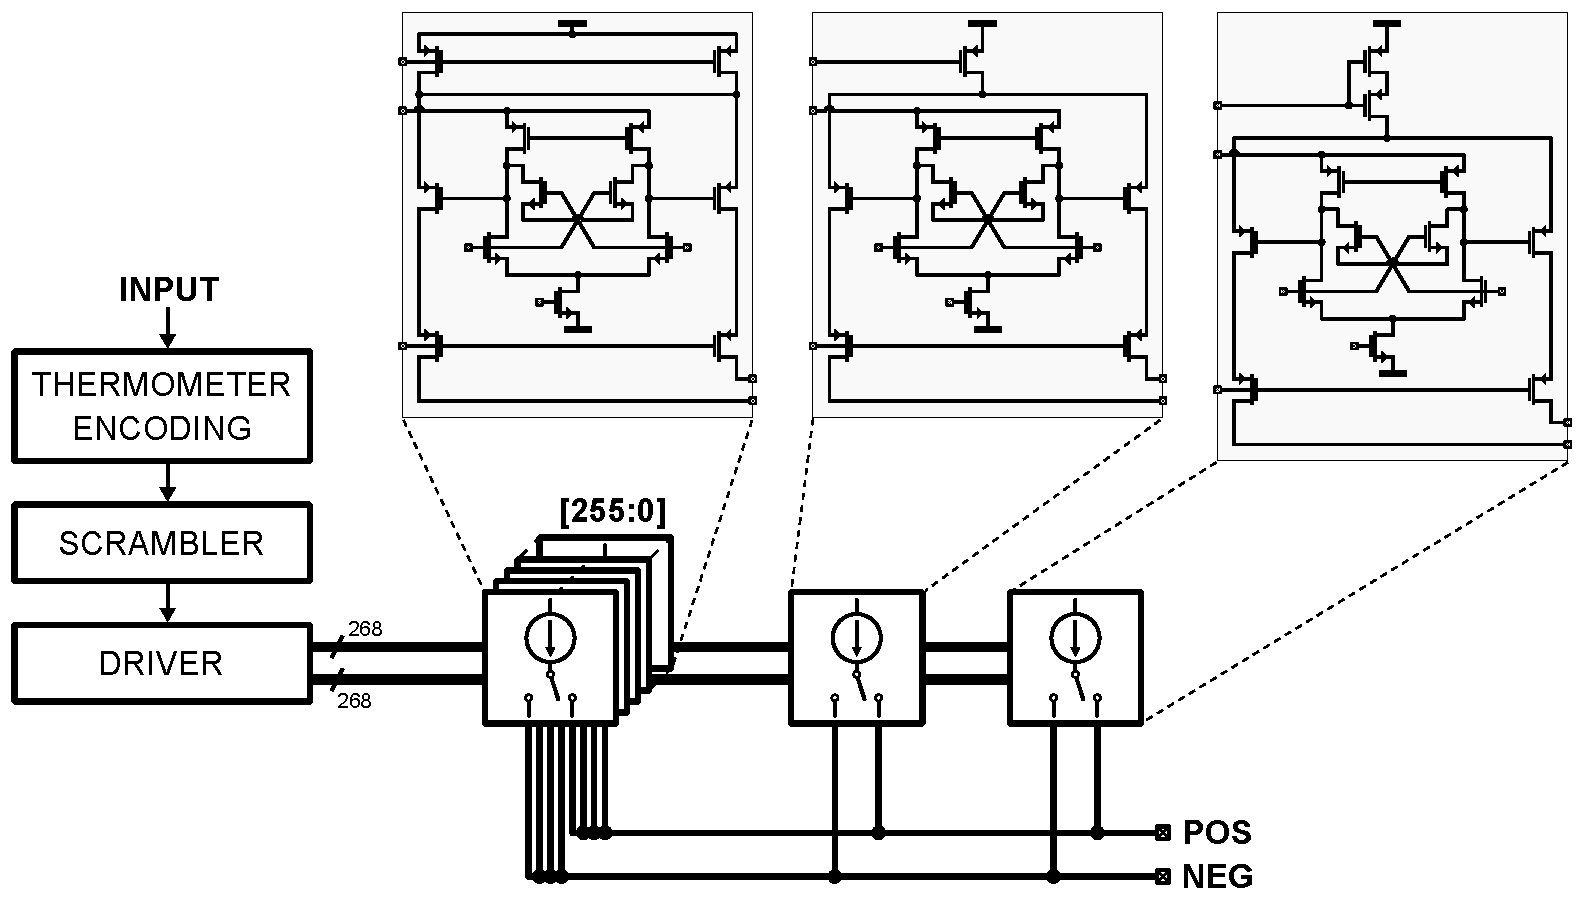
\includegraphics[scale=0.30]{dac_topology.pdf}
}
\end{figure}

\begin{itemize}
 \item 10-bit current steered differential DAC
 \item Mismatch scrambling
\end{itemize}

\end{frame}


%%%%%%%%%%%%%%%%%%%%%%%%%%%%%%%%%%%%%%%%%%%%%%%%%%%%%%%%%%%%%%%%%%%%%%%%%%%%%%%%%%%%%%%%%%%%%%%%%%%%%%%%%%%%%%
\begin{frame}{Mixer Topology}

\begin{figure}[h]
\centering{
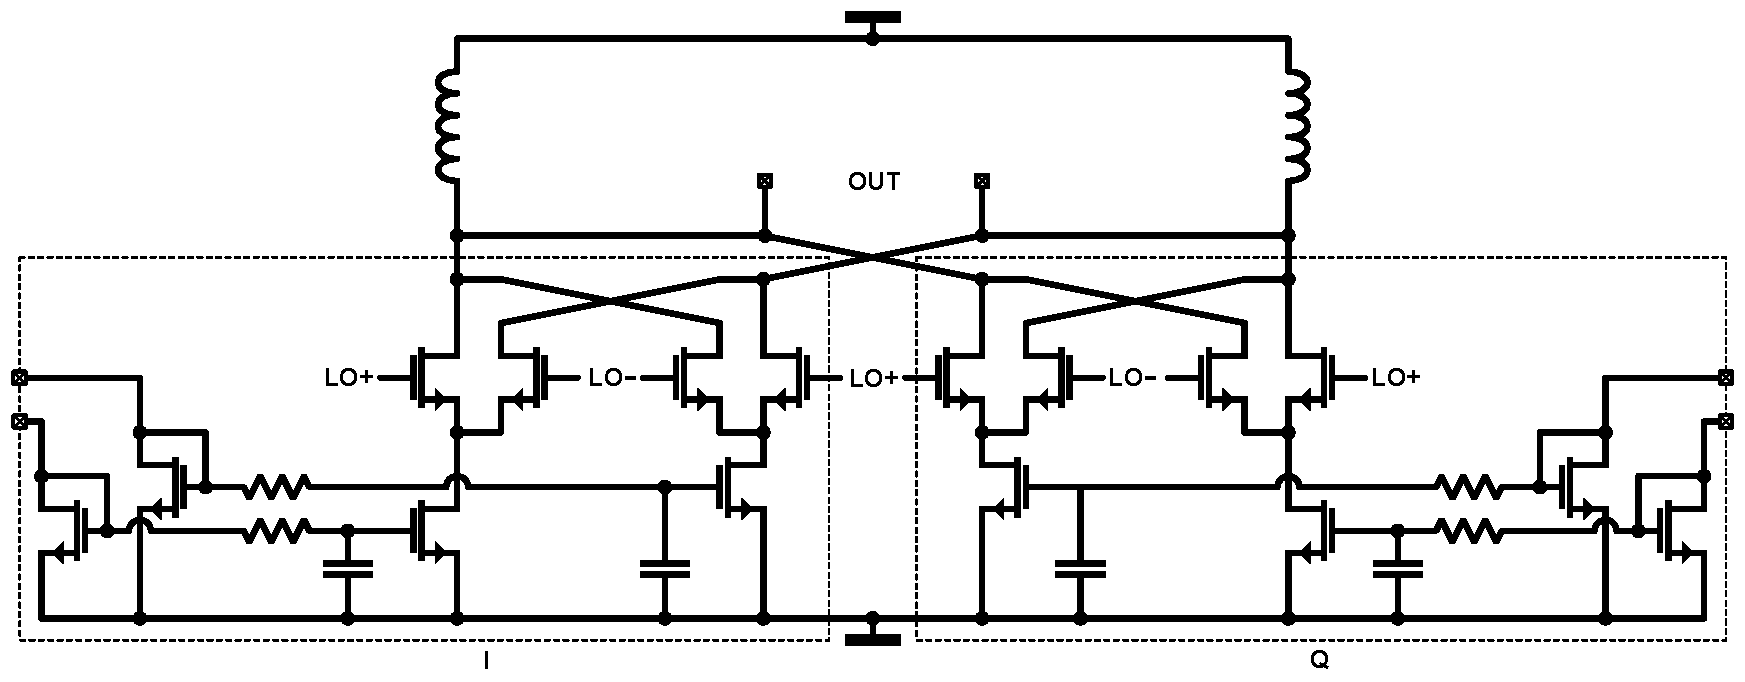
\includegraphics[scale=0.3]{mixer_topology.pdf}
}
\end{figure}

\begin{itemize}
 \item Current inputs
 \item Single pole low pass filter
 \item Baseband to L band
\end{itemize}

\end{frame}


%%%%%%%%%%%%%%%%%%%%%%%%%%%%%%%%%%%%%%%%%%%%%%%%%%%%%%%%%%%%%%%%%%%%%%%%%%%%%%%%%%%%%%%%%%%%%%%%%%%%%%%%%%%%%%
\begin{frame}{Oscillator Topology}

\begin{figure}[h]
\centering{
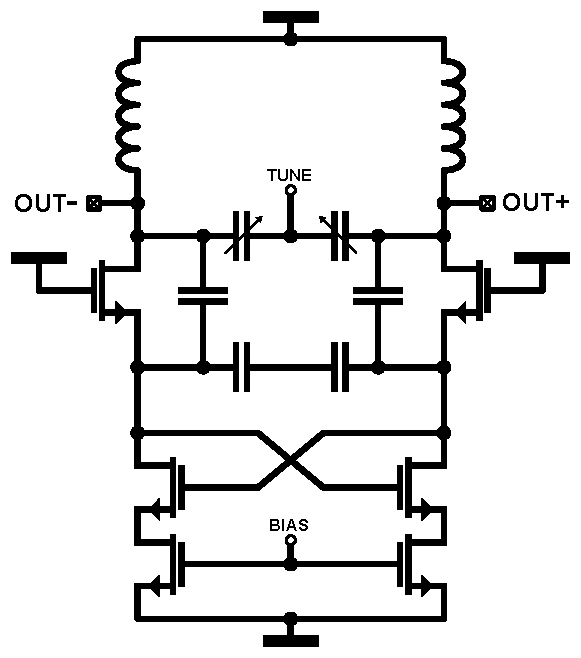
\includegraphics[scale=0.4]{osc_topology.pdf}
}
\end{figure}

\begin{itemize}
 \item Colpitts based topology
 \item 8 GHz nominal
\end{itemize}

\end{frame}


%%%%%%%%%%%%%%%%%%%%%%%%%%%%%%%%%%%%%%%%%%%%%%%%%%%%%%%%%%%%%%%%%%%%%%%%%%%%%%%%%%%%%%%%%%%%%%%%%%%%%%%%%%%%%%
\begin{frame}{DVB-S2(X) Baseband Modulator}

\begin{figure}[h]
\centering{
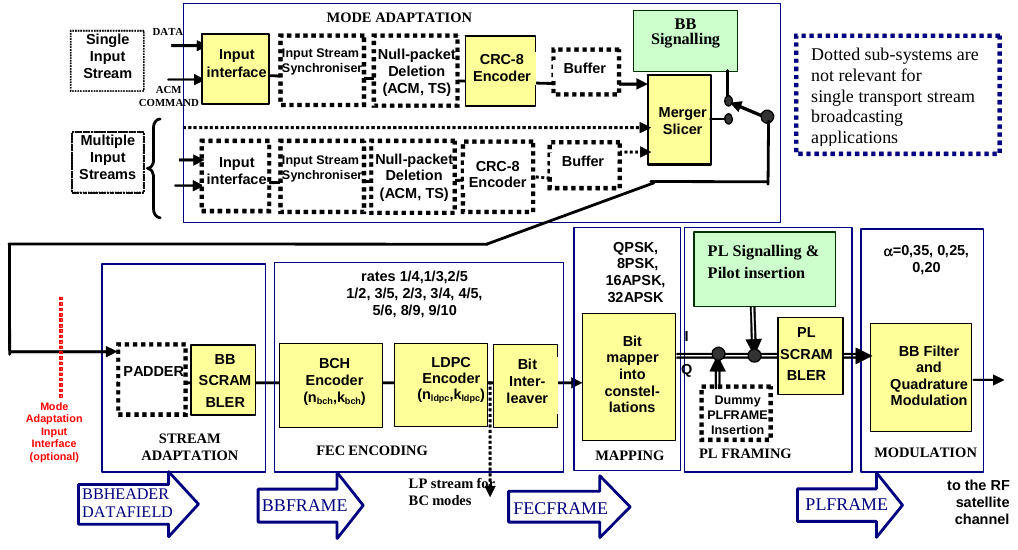
\includegraphics[scale=0.2]{dvb.png}
}
\end{figure}

\begin{itemize}
 \item LDPC + BCH forward error correction
 \item Modulation
 \item Near Shannon limit operation
\end{itemize}

\small Phase4 project: phase4space.github.io

\end{frame}

%%%%%%%%%%%%%%%%%%%%%%%%%%%%%%%%%%%%%%%%%%%%%%%%%%%%%%%%%%%%%%%%%%%%%%%%%%%%%%%%%%%%%%%%%%%%%%%%%%%%%%%%%%%%%%
\begin{frame}{System Goal}

\begin{figure}[h]
\centering{
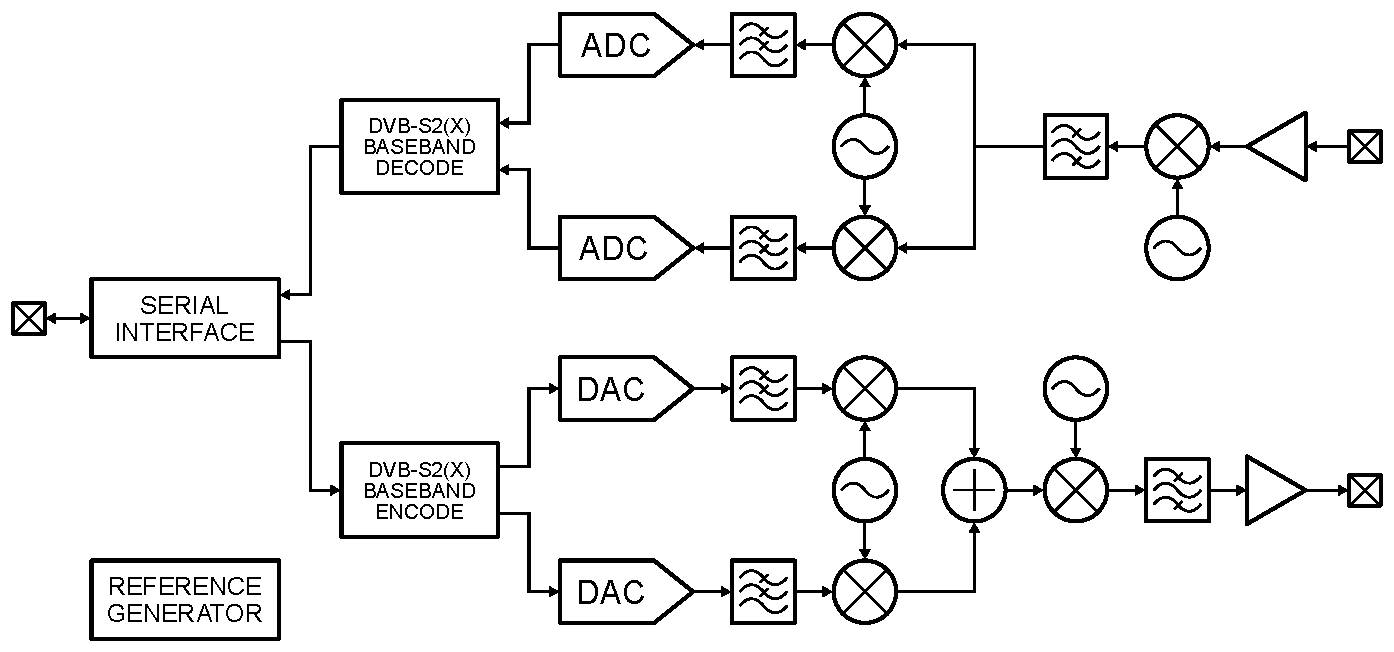
\includegraphics[scale=0.4]{system}
}
\end{figure}

\end{frame}


%%%%%%%%%%%%%%%%%%%%%%%%%%%%%%%%%%%%%%%%%%%%%%%%%%%%%%%%%%%%%%%%%%%%%%%%%%%%%%%%%%%%%%%%%%%%%%%%%%%%%%%%%%%%%%
\begin{frame}{Thanks}

yrrapt@gmail.com

@yrrapt on Skywater Slack channel

\end{frame}



\end{document}